\chapter{Data set}
\label{ch:dataset}
 
%
% Section: 4 - Intro
%
\section{Introduction}
\label{sec:dataset:intro}

Training and evaluation of automatic information extraction approaches requires availability of reliable ground truth data of sufficient size. Following a growth of interest for extraction of information about software tools from scientific publications labeled data sets with limited scope such as BioNerDs, SoftCite, SoSciSoSci have came into existence. More recently, SoMeSci data set, a more comprehensive corpus that covers a wide range of information about software tools has also been introduced \citep{schindler2021somesci}. \\
 
This section presents descriptions about the SoMeSci data set, the extension process of data set with software usage purpose annotations, issues observed during annotation, pre-processing of the data-set, analysis results of the data and transformation to a suitable format for training purpose.  


\section{SoMeSci data set}
\label{sec:dataset:SoMeSci}

SoMeSci data set contains high quality, hand annotated articles collated from PubMed Central (PMC). The articles and annotations included in the data set are summarized below.  

\subsection{ SoMeSci Articles }
\label{subsec:dataset:SoMeSci:Articles}

The corpus is composed four group of files, namely PLoS methods, PLoS sentences, PubMed full text and Creation sentences. Facts about the articles in the SoMeSci corpus is summarized in the table below:

\subsection{SoMeSci Annotations  }
\label{subsec:dataset:SoMeSci:Annotations }

SoMeSci corpus has three main types of annotations that correspond to a type of information related with software tools. These annotations indicate the type of software, type of mention and additional information about the software as summarized on the table below:


\section{Annotation tool}
\label{sec:dataset:tool}
The data set has been annotated using BRAT rapid annotation tool, v.1.3 , in a Linux 20.4 environment. The annotation tool has been run in a local machine as a CGI application using a browser. 

\begin{figure}[htbp]
	\centering
	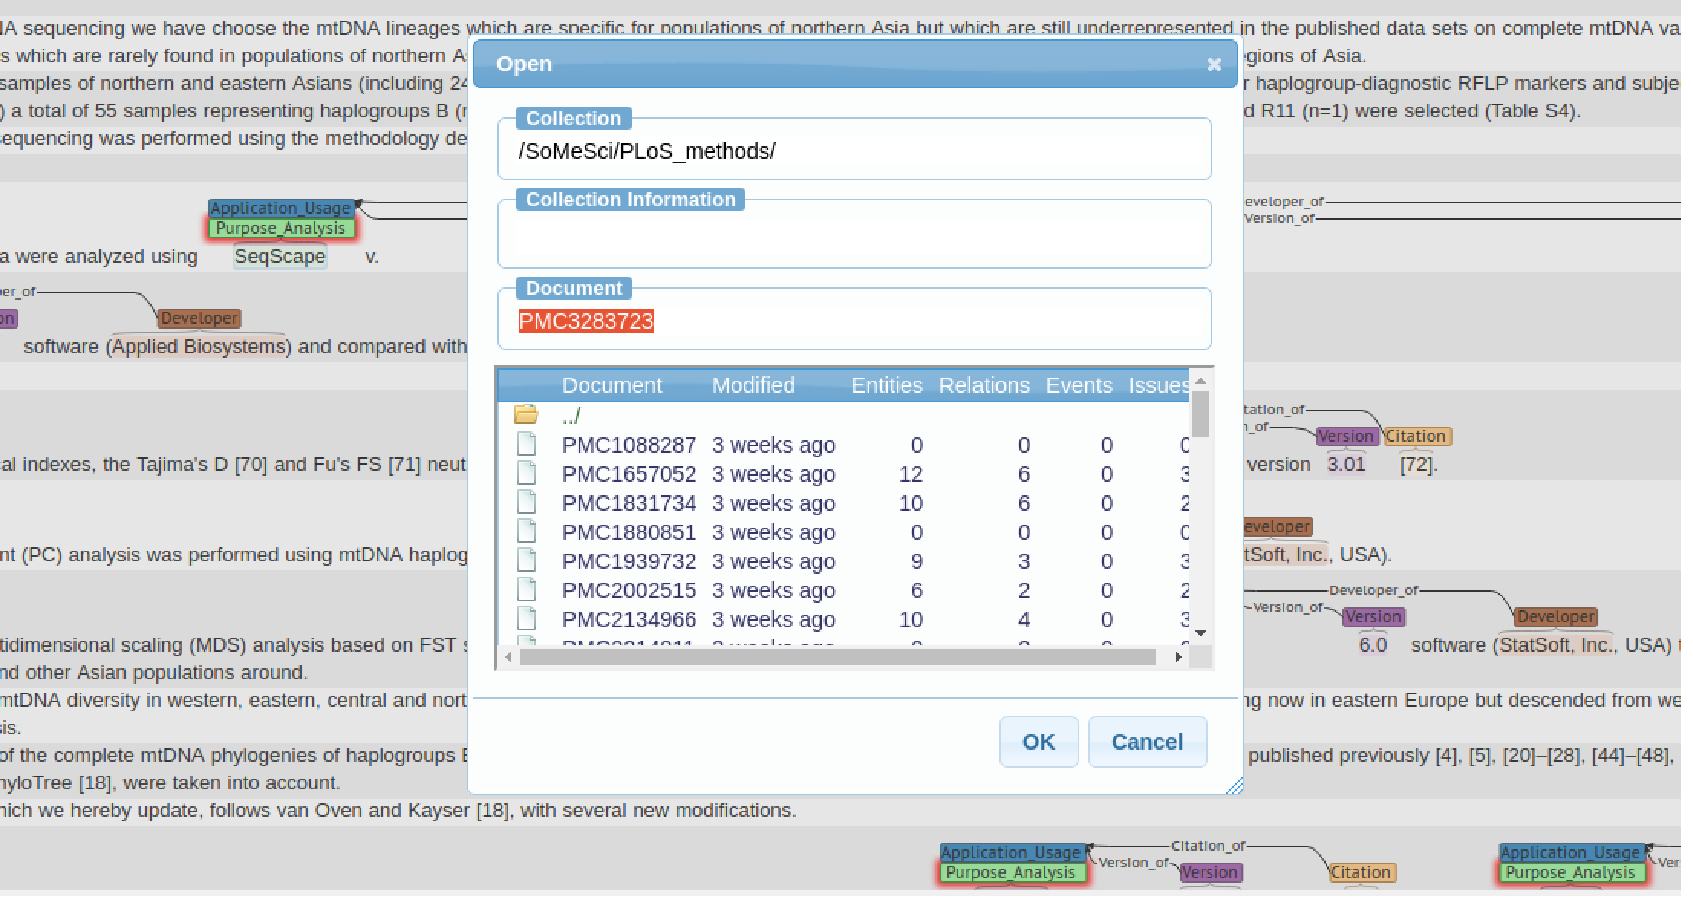
\includegraphics[width=.75\textwidth]{4.graphics/figures/models/pdf/BRAT_tool}
	\caption{Workflow for identifying software purposes}
	\label{fig:chapter04:setup}
\end{figure}

\subsection{Annotation of SoMeSci with software purpose labels}
\label{subsec:dataset:tool:Annotationprocess}

SoMeSci corpus has been extended with annotations of eight classes of purpose of software usage labels identified in the earlier section. Since using software for a particular purpose only refers to the usage of a software, only usage labels has been further labelled with software purpose. The figure below shows SoMeSci data set before and after software purpose annotations. \\

\subsection{Challenges during Annotation }
\label{subsec:dataset:tool:Challenges}
Annotations has been carried out in a such way by deciding on each context which software purpose annotation is more important or based on the general goal of the software usage. For example, FlexArray software on the figure below, has been annotated with software purpose analysis even though the same software was used for visualization purpose as well. This is because on this context analysis is more important than visualization and essentially visualization could also be interpreted as one kind of analysis. In addition, specific definition of each of software usage purposes has been also taken into account. \\

However, annotation of software usage statements was not often straightforward. This is because, in some instances as shown in the figure below, purpose of software usage might not be clear from the context.\\

In addition in some cases possibility of multiple candidate labels for a given software usage label was also observed. For example  

The other challenge of annotation was difficulty arising from limited domain knowledge. 

\section{Data Pre-processing}
\label{sec:dataset:preprocessing}
Pre-processing of the data set has been carried out to ensure the integrity of our data set before using it in the classifier. The data pre-processing tasks handled annotation errors, merging annotations , transforming and splitting of data set. 

\subsection{Handling missing annotations and annotation errors }
\label{subsec:dataset:preprocessing:handlingerrors}

During the first phase  annotation of SoMeSci usage mentions, few instances where  the original software usage annotation seemed like just mention of software has been skipped. Hence, pre-processing of the data set has been carried out to ensure the integrity of the overall annotation by automatically identifying software usage instances that are not annotated and erroneous annotation of other types of software mentions other than software usage. \\

After identifying the list of files and instances of annotations with an error or skipped annotations, all errors have been rectified and skipped annotations has been handled.


\subsection{Merging annotations}
\label{subsec:dataset:preprocessing:Merging}


After handing all annotation errors and missing labels, annotations of software usage has been merged with annotations of software purpose. Merging of the annotations solves two problems. \\

First it will fix annotation error message that is displayed on the BRAT tool. The error message is displayed because more than one annotation per a token is not supported by the annotation tool. \\

The other reason for merging annotations is to take advantage of legacy code, ariclenizer, which will transform data from BRAT too in a stand-off format  into IOB format which is desirable for training purpose. 

\begin{figure}[htbp]
	\centering
	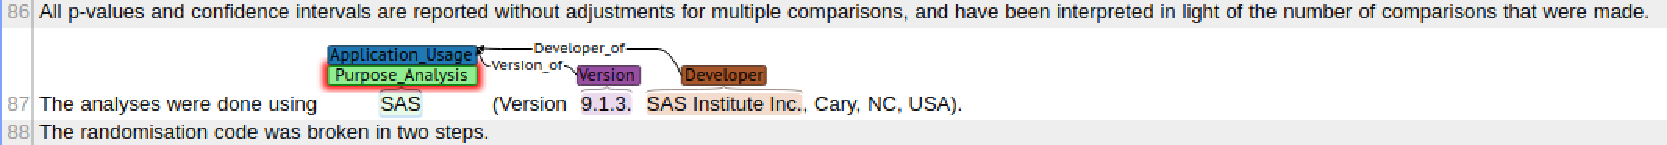
\includegraphics[width=1\textwidth]{4.graphics/figures/chap4/merging/2002515_plm_unm}
	
	\label{fig:chapter04:setup}
\end{figure}

\begin{figure}[htbp]
	\centering
	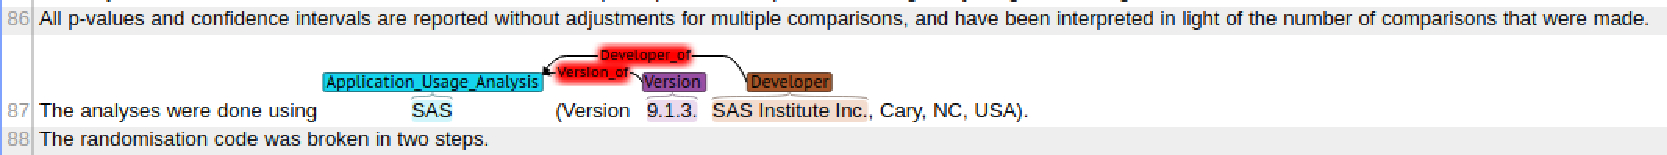
\includegraphics[width=1\textwidth]{4.graphics/figures/chap4/merging/2002515_plm}
	\caption{Annotations before merging and after.}
	\label{fig:chapter04:setup}
\end{figure}




\subsection{Transformation to IOB format}
\label{subsec:dataset:preprocessing:Transformation}
After merging software usage and purpose labels, transformation of data into IOB format has been carried out using articlenizer (link to articlenizer). Picture below shows the data format before and after transformation. 

\begin{figure}[htbp]
	\centering
	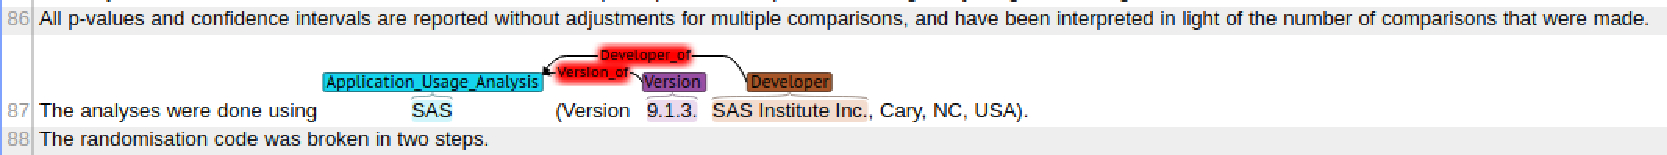
\includegraphics[width=1\textwidth]{4.graphics/figures/chap4/merging/2002515_plm}
	
	\label{fig:chapter04:setup}
\end{figure}

\begin{figure}[htbp]
	\centering
	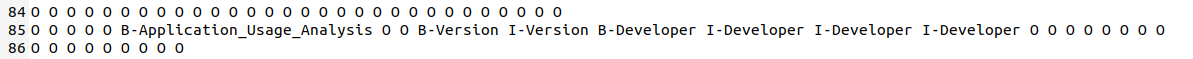
\includegraphics[width=1\textwidth]{4.graphics/figures/chap4/merging/BIo_2002515_plosmeth}
	\caption{A sentence in BIO format after BIO transformation.}
	\label{fig:chapter04:setup}
\end{figure}

\subsection{Data Splitting}
\label{subsec:dataset:preprocessing:Splitting}
After the data has been transformed into the IOB format, it has been further split into training, development and test set in 60:20:20 ratio.


\section{Analysis of Annotated Data}
\label{sec:dataset:Analysis}

Analysis of cleaned SoMeSci data set has been carried out to find a deeper insight about the training data. 

\subsection{Co-reference resolution of software entities }
\label{subsec:dataset:Analysis:resolution}

The base line for the analysis of the data set was to carry out disambiguation of software names. This was particularly important because there is large degree of variation in software names. Using list of software name with corresponding URL, software mention instances have been disambiguated from each other and all software name variations that refer to the same entity have been given the same name. Figure below shows name variations for MATLAB software, in which all instances resolve to the same URL i.e. entities referring to the same software. All variations of names has been replaced by the first “Matlab” in this case.


\subsection{Analysis results }
\label{subsec:dataset:Analysis:results}

According to the analysis results, the top 3 software by number of software name mention count through out the list of articles in PubMed and PLoS data set are: PASW, GNU-R and STATA.  

\begin{figure}[htbp]
	\centering
	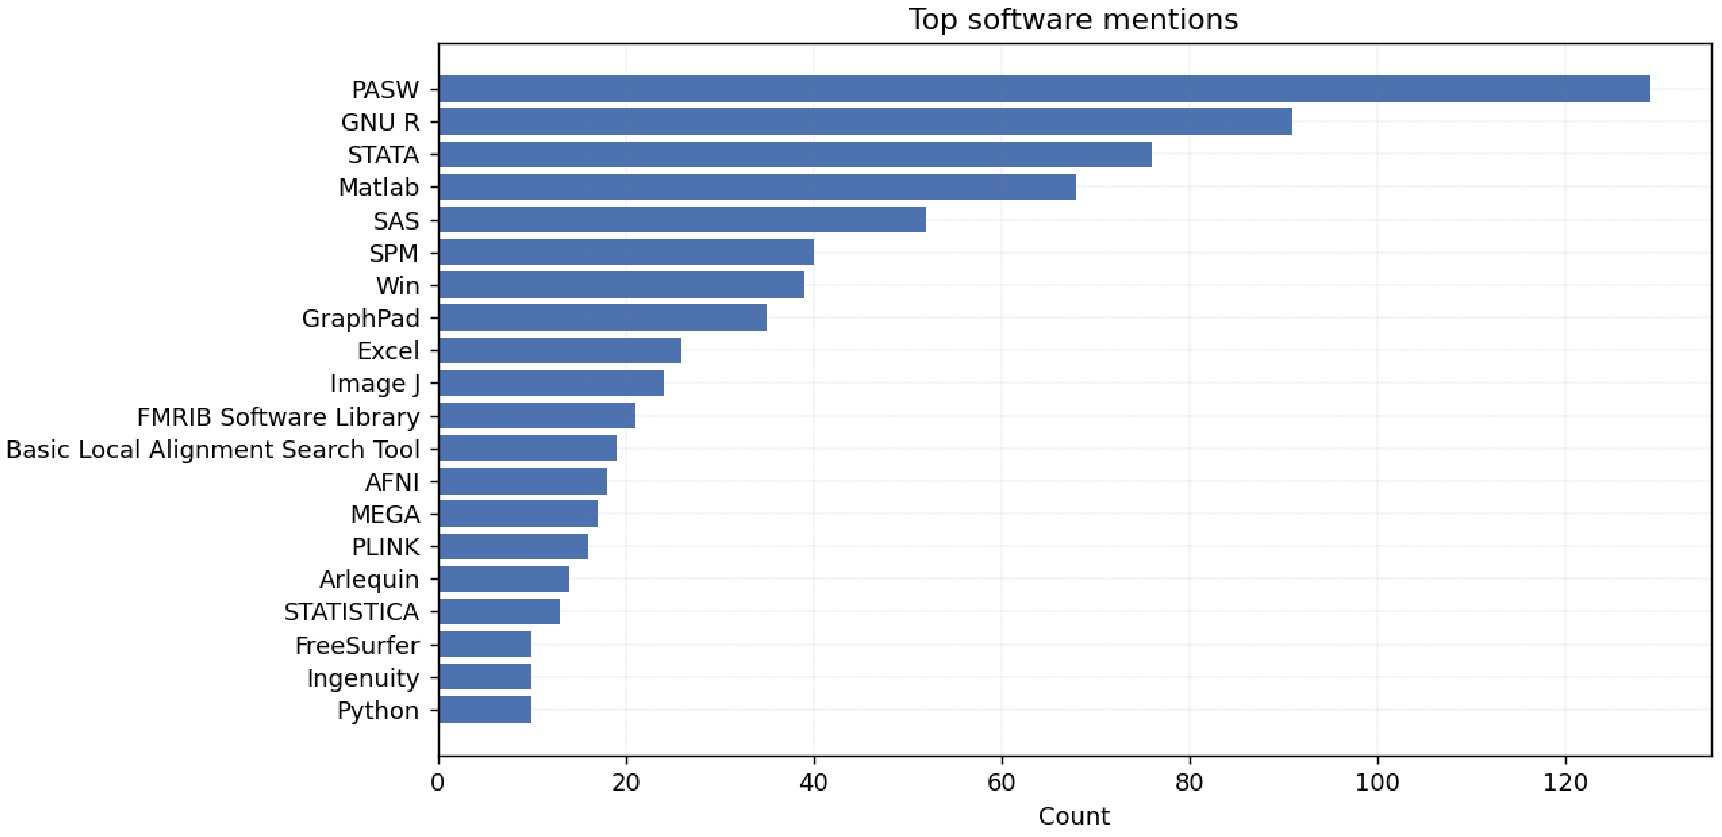
\includegraphics[width=1\textwidth]{4.graphics/figures/analysisresults/1.Top software mentions}
	\caption{Top software mentions}
	\label{fig:chapter03:setup}
\end{figure}

Data set analysis result from the perspective of purpose of software usage indicates that, the most common purpose of software usage are: Analysis, Data pre-processing, Data collection and modelling where as the least common are simulation and stimulation. 

\begin{figure}[htbp]
	\centering
	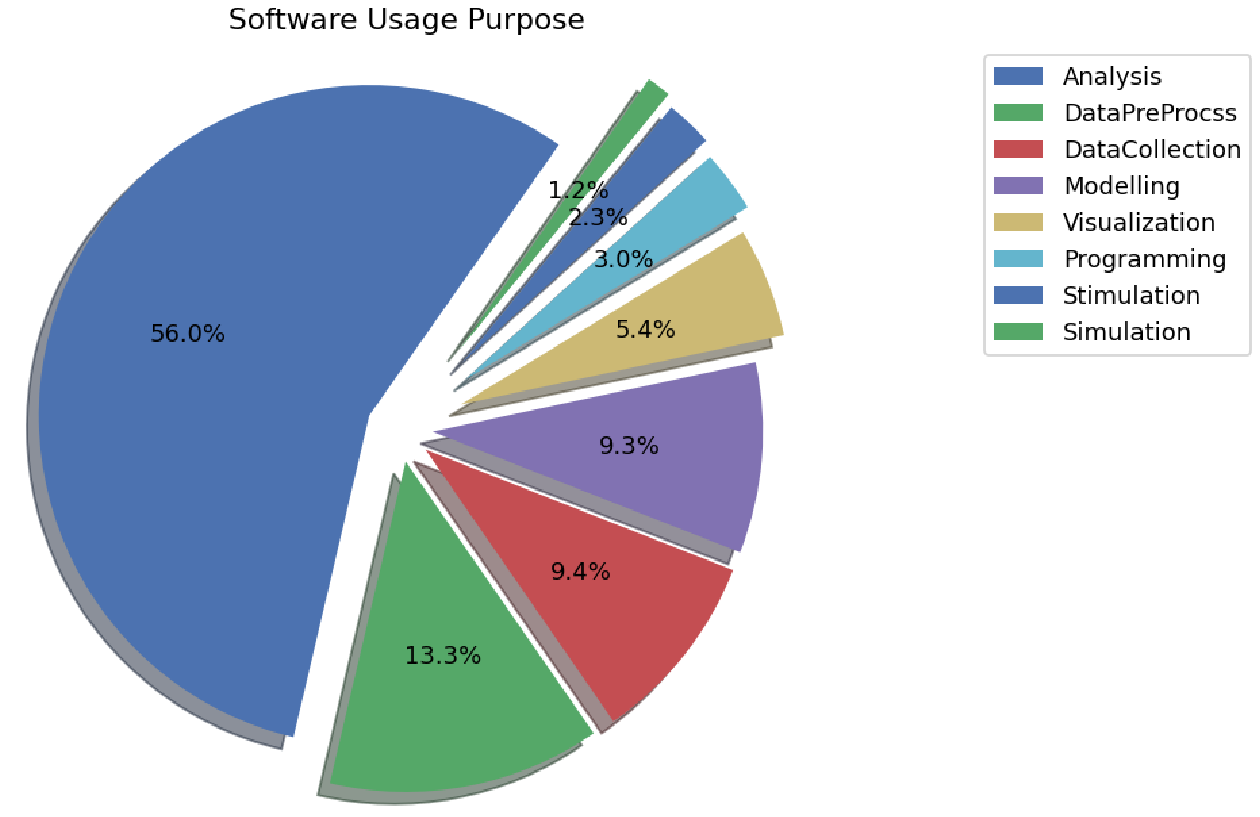
\includegraphics[width=.65\textwidth]{4.graphics/figures/analysisresults/2.Software Usage Purpose pie}
	\caption{Top software usage purposes}
	\label{fig:chapter03:setup}
\end{figure}

\begin{figure}[htbp]
	\centering
	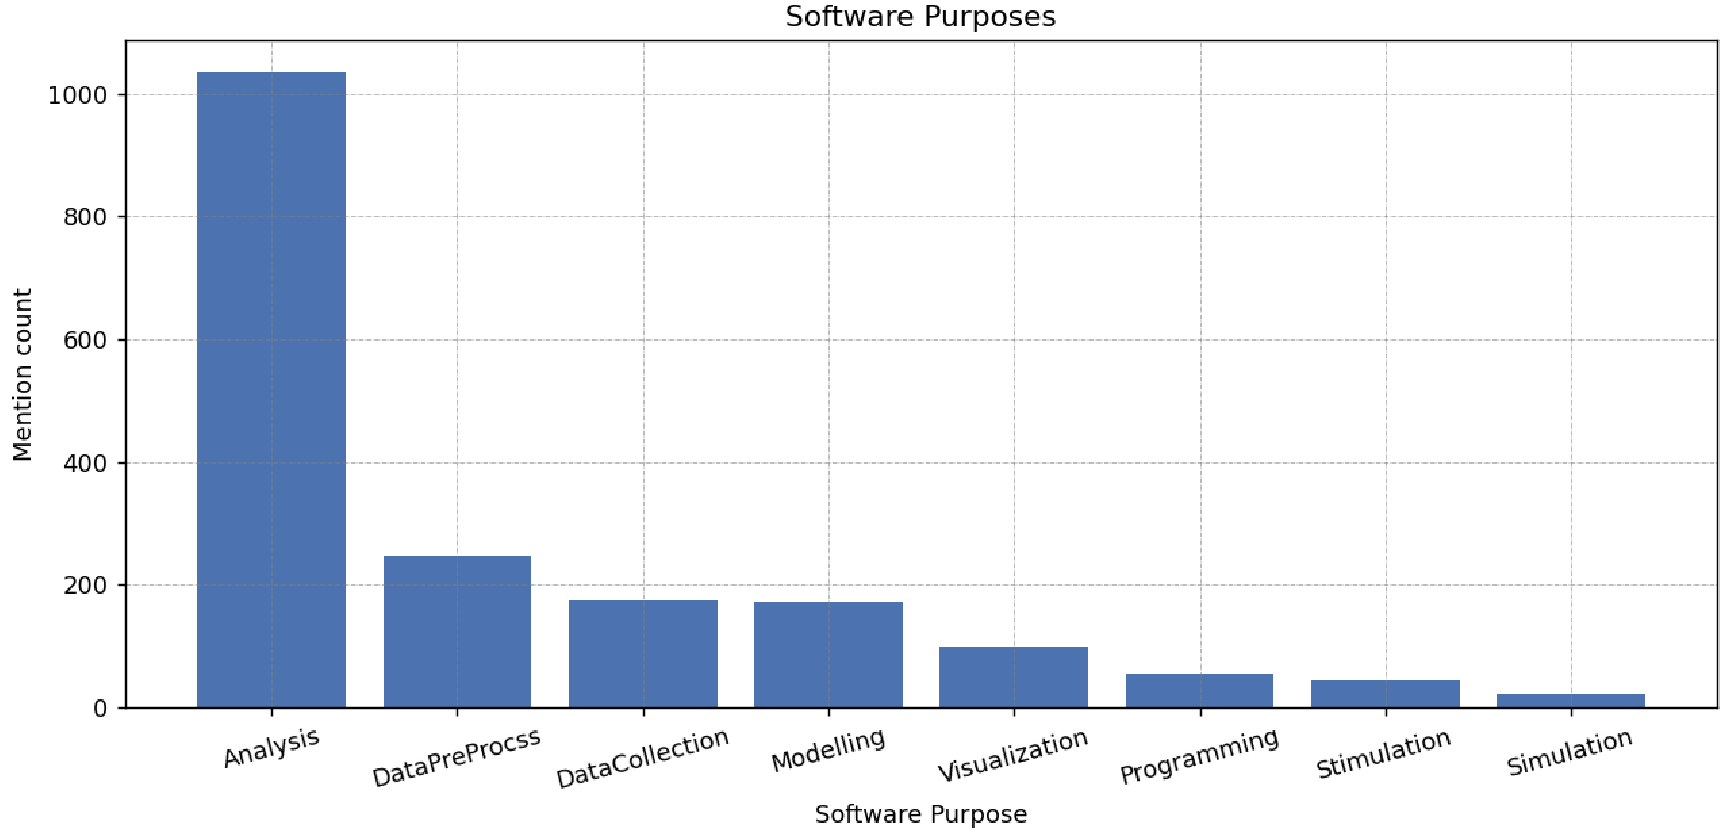
\includegraphics[width=1\textwidth]{4.graphics/figures/analysisresults/3.Software Purposes}
	\caption{Top software usage purposes}
	\label{fig:chapter03:setup}
\end{figure}

The other insight form from  the software-type perspective, is that the most commonly used type of software in the research articles in the data set is Application software.  


\begin{figure}[htbp]
	\centering
	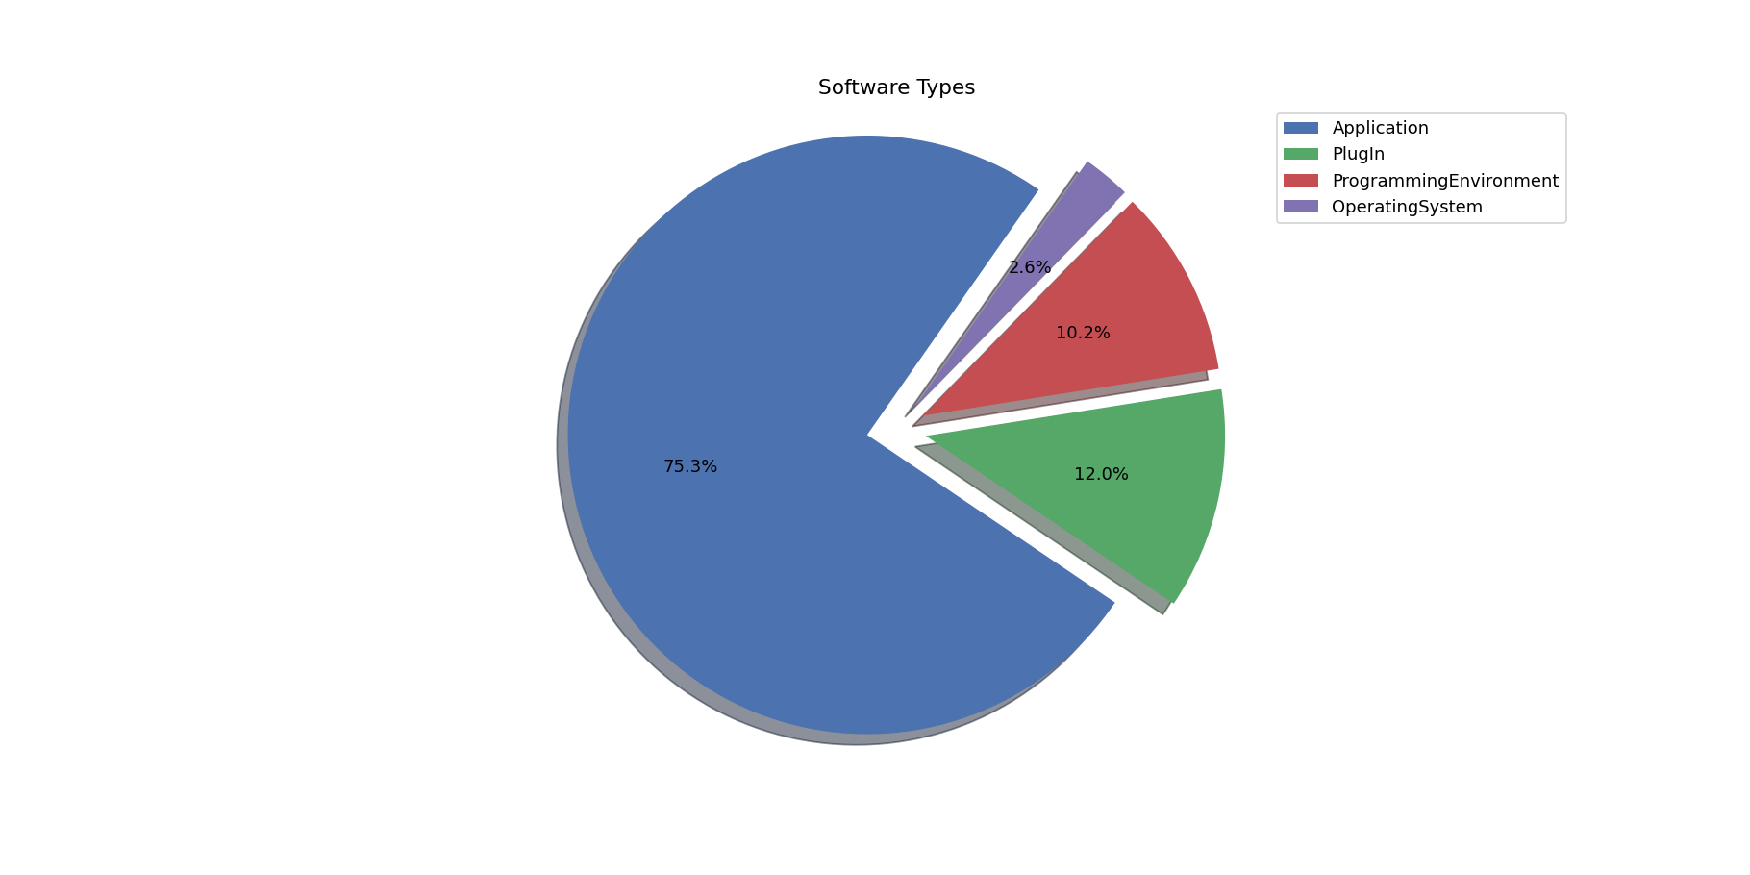
\includegraphics[width=.65\textwidth]{4.graphics/figures/analysisresults/4.Software Types pie}
	\caption{Software types}
	\label{fig:chapter03:setup}
\end{figure}

When it comes to share of each purpose of software usage among the 4 types of software, the pattern once again clearly indictaes most of the time a software has been used for the purpose of analysis and data collection in all of the four software types. 

\begin{figure}[htbp]
	\centering
	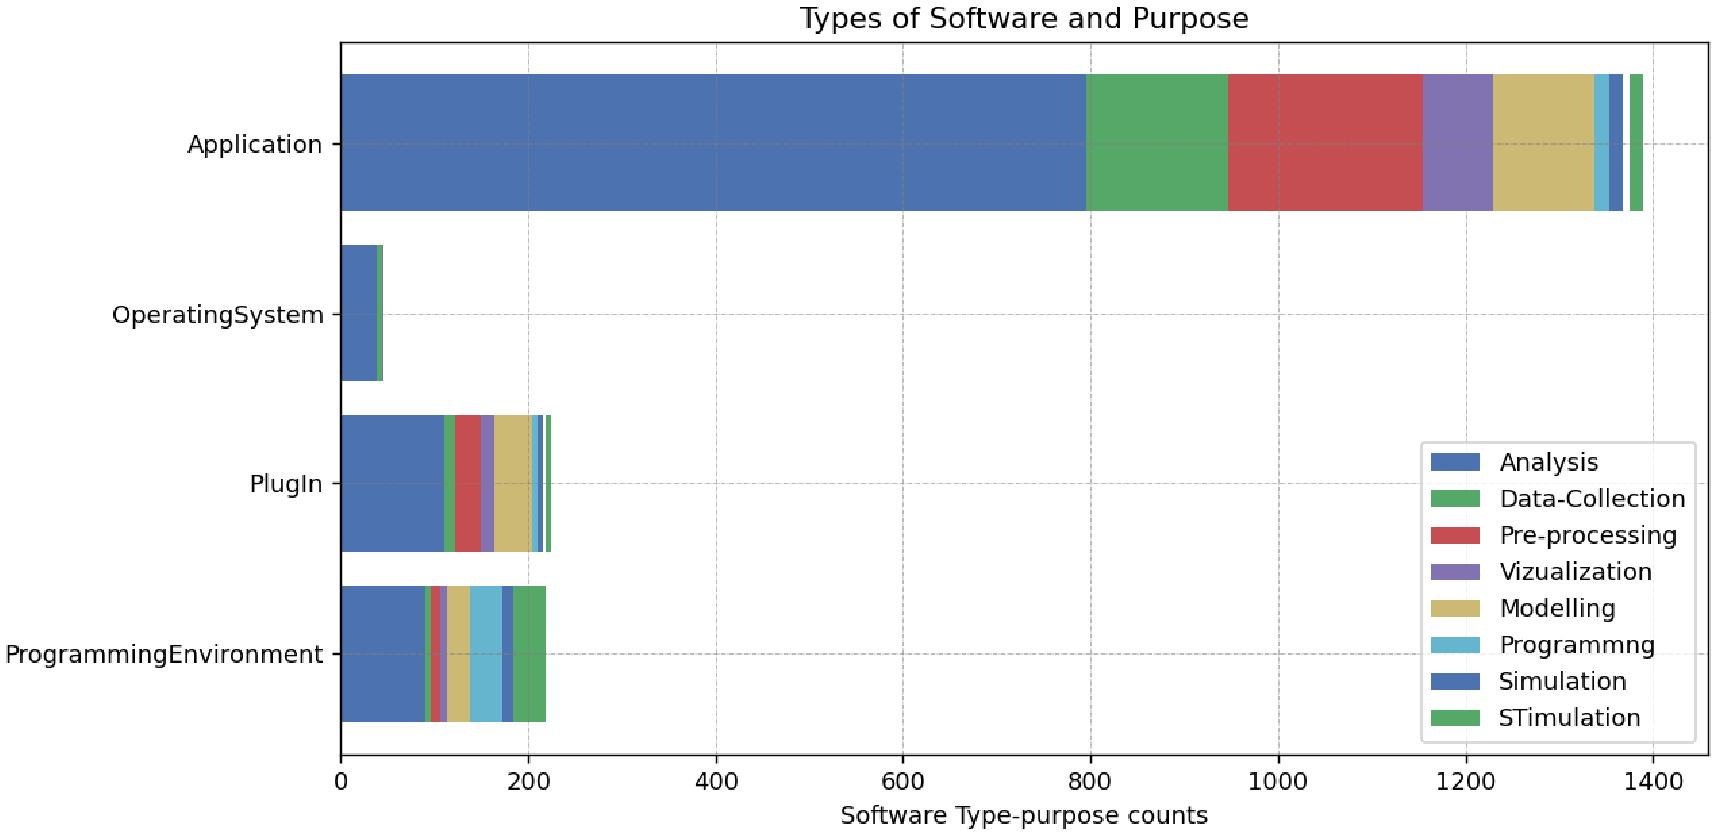
\includegraphics[width=1.1\textwidth]{4.graphics/figures/analysisresults/6.Types of Software and Purpose stacked bar}
	\caption{Software types and purposes}
	\label{fig:chapter03:setup}
\end{figure}

Lastly, the most interesting insight that is important for the automatic classification task was determining: ” for how many different purposes a given software have been used for ?”.  The analysis result reveals that from 657 unique software lists, a little over 3 out of 4 software have been used only for a single purpose. Over all almost 98\% of software have been used for a purposes maximum of three. This indicates that most of the software have been used only for a specific purpose.  

\begin{figure}[htbp]
	\centering
	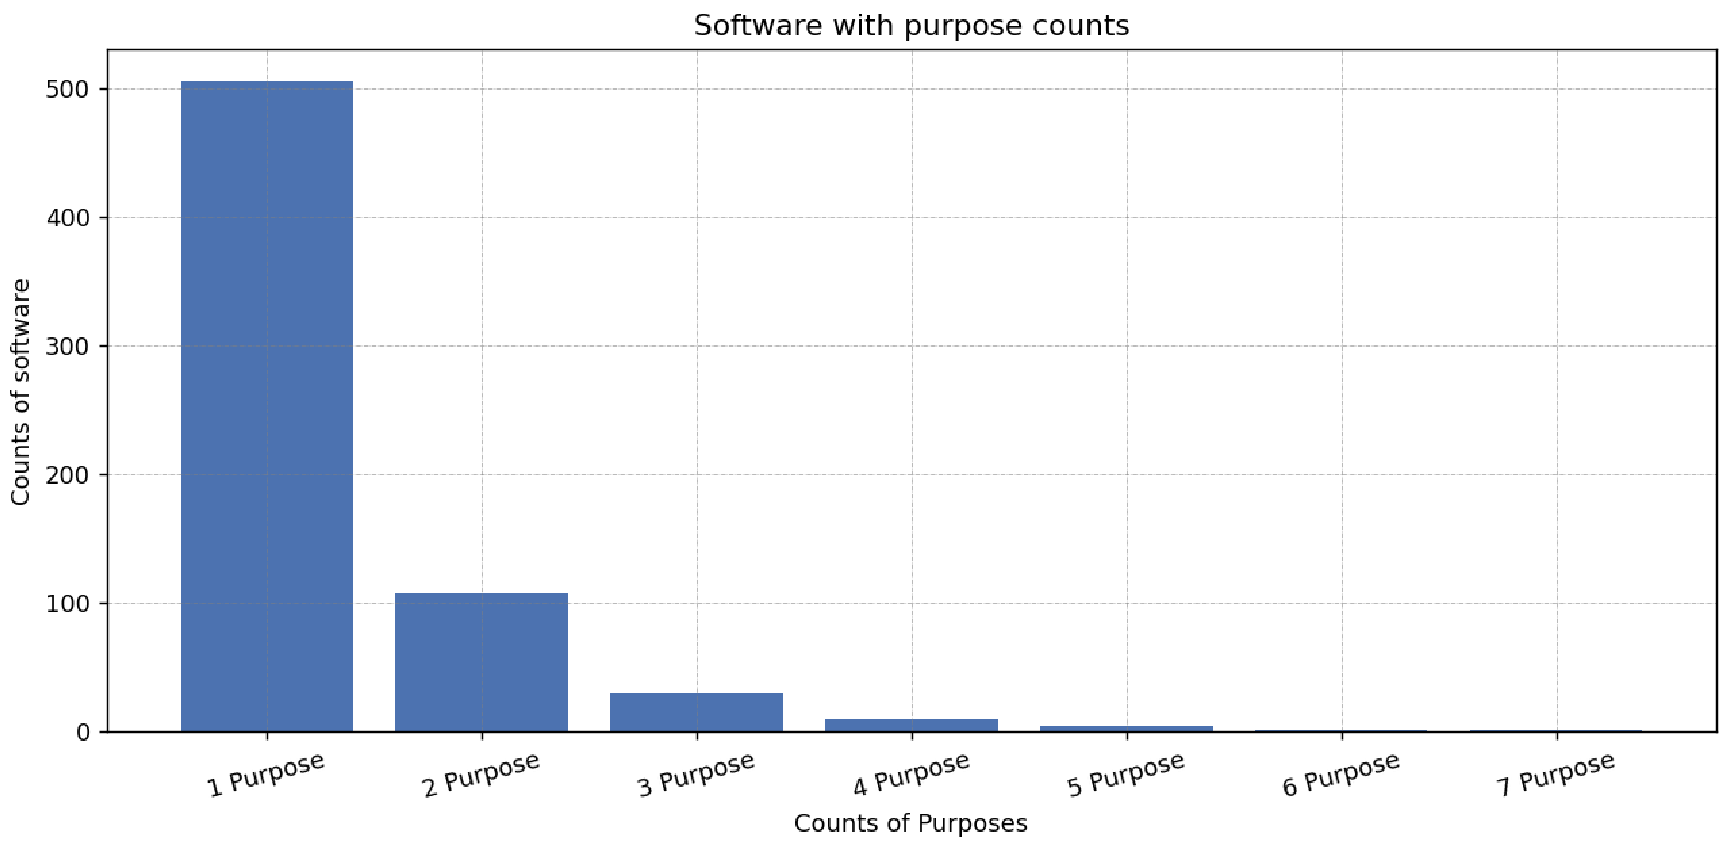
\includegraphics[width=1\textwidth]{4.graphics/figures/analysisresults/7.counts of software purpose}
	\caption{Software purposes counts}
	\label{fig:chapter03:setup}
\end{figure}

\begin{figure}[htbp]
	\centering
	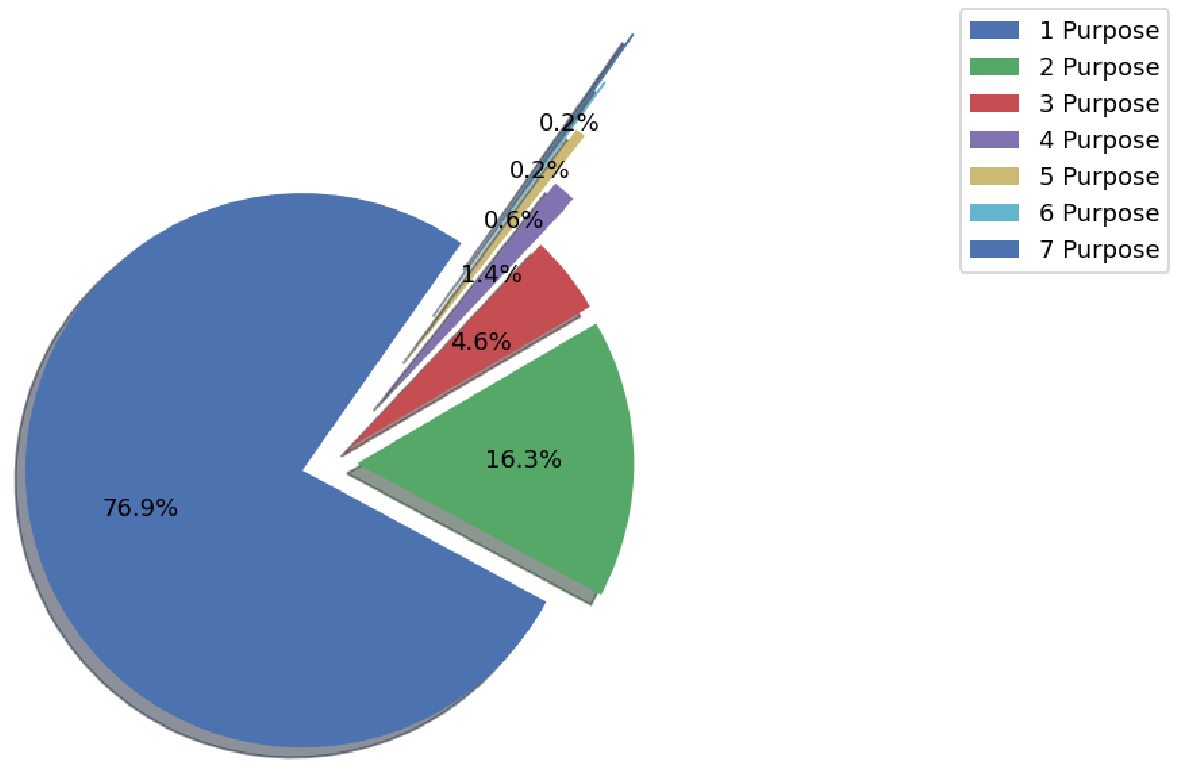
\includegraphics[width=.65\textwidth]{4.graphics/figures/analysisresults/8.counts of software purpose pie}
	\caption{Software purposes }
	\label{fig:chapter04:pie}
\end{figure}

\section{Summary }
\label{subsec:dataset:Analysis:Summary}

This section has described the training data set, the annotation process and insights about the data. One of the core results of the analysis result is the fact that most of the time, software has been used for a specific purpose[write this in the results]. The next section presents models that could be suitable for classification of purpose of software usage statements using the data set described above. 

